%# -*- coding: utf-8-unix -*-
%%==================================================
%% chapter01.tex for SJTU Master Thesis
%%==================================================

%\bibliographystyle{sjtu2}%[此处用于每章都生产参考文献]
\chapter{开源混合存储系统分析}
\label{chap:opensource_intro}

目前,开源的混合存储系统中被使用较为广泛的是flashcache、dm-cache、bcache这三个系统,但是对于这三个系统的研究主要集中在对他们的算法研究\cite{杨宗2013flashcache, 唐华敏2015bcache},而对他们的对比较少。本章将首先对flashcache、dm-cache、bcache这三个开源混合存储系统分别从系统架构、数据映射策略、冷热数据识别策略、数据写回/迁移策略、最优化存储设备组合进行介绍,然后对他们从性能和特性两方面进行对比分析。

\section{flashcache}

\subsection{系统架构}

flashcache基于device mapper,采用分层架构,将缓存设备与后台设备统和为一块逻辑设备,缓存设备作为后台设备的数据缓存。

\subsection{数据映射策略}
\label{sec:flashcache_mapping}
flashcache采用块级映射策略中的组关联映射规则,通过set associative hash\cite{kimmel2014set}将缓存设备分成多个固定大小的set(一个set默认为512个block)并组织起来,将请求的block的起始扇区(dbn)通过公式\ref{eq:dbn_to_set}映射到target set,再在target set内部进行线性探测获取block,如图\ref{fig:flashcache_map}所示。

\begin{equation}
    \label{eq:dbn_to_set}
    target \ set = \frac{dbn}{block size \times set size} mod (set \  number)
\end{equation}

\begin{figure}[!htp]
    \centering
    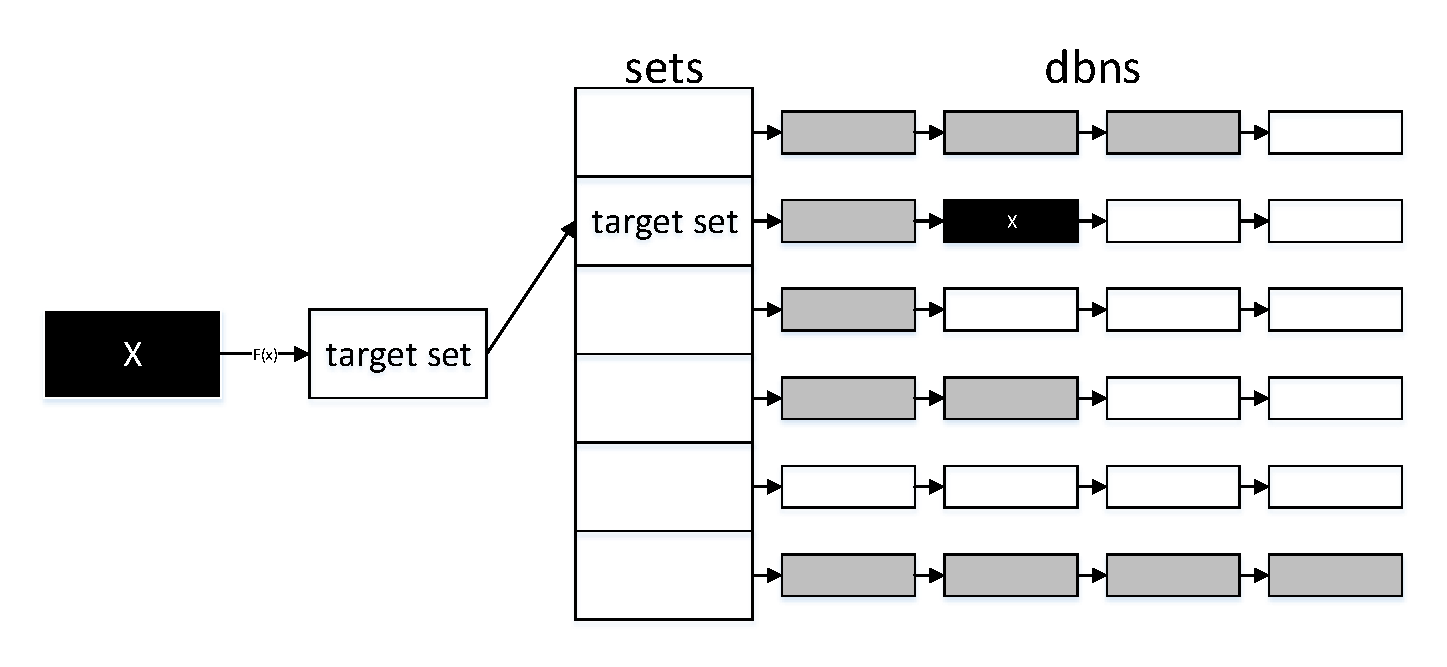
\includegraphics[width=0.8\textwidth]{flashcache_map.pdf}
    \bicaption[fig:flashcache_map]{flashcache的组相联映射}{flashcache的组相联映射}{Fig.}{group mapping in flashcache}
\end{figure}

\subsection{冷热数据识别策略}

flashcache以块级对数据进行冷热识别,采用双层lru链表结构将数据分为频繁访问的数据、偶尔访问的数据以及冷数据,如此一来,大量的遍历型I/O请求并不会导致大量的缓存失效,并且flashcache支持识别顺序性读写请求并略过对顺序性读写请求中数据的缓存操作。

\subsection{数据写回/迁移策略}

flashcache在每次I/O调用及每次I/O调用的回调时触发将脏数据从缓存设备写回到后台设备,并限制每次写回的脏数据的块数量,因此可以稳定地刷出脏数据而不会造成系统的负载突发性增长,另外可以设置将所有脏数据强制全部写回。

\subsection{最优化存储设备组合}

flashcache采用静态策略,并且限制缓存设备与后台设备都只能有一个。

\section{dm-cache}

\subsection{系统架构}

dm-cache基于device mapper,采用分层架构,将缓存设备与后台设备统和为一块逻辑设备,缓存设备作为后台设备的数据缓存。

\subsection{数据映射策略}

dm-cache采用Extent级映射策略,将缓存设备分成大小固定的缓存块(缓存块大小为32KB的整数倍),缓存块通过hash表组织避免了set associative hash的利用率低和冲突问题。

\subsection{冷热数据识别策略}

dm-cache最初使用multi queue对冷热数据进行管理与识别,最新的则是对multi queue进行优化,使用smq(stochastic multi queue,随机多队列模式)对缓存块进行管理。smq本质就是一个多层lru算法,最多可以有64层,层数代表数据的冷热程度不同。smq并不记录缓存块的命中数,并根据命中数记录在不同层,因为这样会导致命中数越是高的层记录的缓存块越少而命中数越少的层记录的缓存块越多,最终导致层与层之间不平衡。smq在缓存块命中时将该缓存块与它上层中最近最少使用的缓存块进行交换,达到不同层平衡的效果。

\subsection{数据写回/迁移策略}

dm-cache在每次I/O调用时触发将脏数据从缓存设备写回到后台设备,并限制通过阈值限制每秒写回的脏数据块数。

\subsection{最优化存储设备组合}

dm-cache采用静态策略,并且限制缓存设备与后台设备都只能有一个。

\section{bcache}

\subsection{系统架构}

bcache没有采用device mapper而是自己实现了一套系统,采用分层架构,将缓存设备与后台设备统和为一块逻辑设备,缓存设备作为后台设备的数据缓存。

\subsection{数据映射策略}

bcache采用Extent级映射策略,将缓存设备分成大小固定的bucket(默认512KB),bucket内部空间采用追加分配的方式,记录当前的偏移量,下次分配时从当前偏移量继续向后分配,数据映射到bucket时主要有2个考量:优先将连续的数据映射到同一个bucket中即使他们可能来源于不同进程的I/O操作;优先将同一进程操作的数据映射到同一bucket中。bucket通过B+树进行管理,每个树节点内部为4个bset结构,每个bset存有排好序的bkey。

\subsection{冷热数据识别策略}

bcache在每个bucket中记录16位长的优先级,每次bucket命中,优先级加一,同时所有bucket的优先级周期性减少,bcache通过bucket的优先级实现lru算法进行冷热数据的识别。

\subsection{数据写回/迁移策略}

bcache当bucket使用超过阈值时会触发垃圾回收,或者当用作缓存的缓存设备容量不够时直接集中写回到后台设备,这一操作会耗费大量CPU(遍历btree)和触发大量后台设备I/O操作。

\subsection{最优化存储设备组合}

bcache采用动态策略,虽然限制缓存设备只能有一个,但支持多个后台设备并且在运行中动态增加。

\section{对比分析}

flashcache、dm-cache、bcache经过测试后的特性对比如下所示。

\subsection{可靠性}

flashcache的可靠性较高,采用分散式刷脏数据策略(控制刷脏数据速率),所以在I/O重负载的情况下系统不会表现为无法响应的状态,表现优秀。当作为缓存的SSD满后,且数据没有重叠时会击穿缓存,直接访问磁盘。 

dm-cache的可靠性较弱,在I/O重负载的情况下系统会因为刷脏数据无法响应,但是因为刷脏数据的效率较高,所以未响应表现为间歇性。当作为缓存的SSD满后,且数据没有重叠时会击穿缓存,直接访问磁盘。 

bcache的可靠性弱,在I/O重负载的情况下系统会长时间无法响应,因为是按bkey遍历树刷出,刷脏数据比较慢,所以系统未响应时间很久,不可控。当作为缓存的SSD满后,且数据没有重叠时会击穿缓存,直接访问磁盘。

\subsection{被缓存的数据大小}

flashcache严格按照缓存块大小进行缓存,不符合条件即大小不一致或边界未对齐的读写请求都不会进行缓存。

dm-cache缓存块采用固定大小,但是当小于设置的缓存块大小时也会被缓存,模块会先从后台设备上把数据迁移到作为缓存设备中,然后进行I/O操作。 

bcache可以缓存任意大小的数据。用bkey追踪,放入树中,因此可能会产生大量的小块。

\subsection{内存开销}

flashcache每个缓存块占用25字节空间,假设被用作缓存的SSD大小为20GB,当缓存块大小设置为4KB时,内存占用约为110MB,在缓存块大小同样的情况下,内存占用和用作缓存的SSD的容量大小基本成正比。  

dm-cache每个缓存块占用24字节空间,假设被用作缓存的SSD大小为20GB,当缓存块大小设置为4KB时,内存占用约为105MB,在缓存块大小同样的情况下,内存占用和用作缓存的SSD的容量大小基本成正比。

bcache占用的内存大小难以直接估计,与用来存元数据的bucket的数量相关,当缓存设备容量较大的时候,这个值会很大(假设缓存大小为26GB,块大小设置为4KB,则大概占用600MB的内存)。树动态增长,树节点数只增不减,当内存不足时,会触发回收,但是查看节点状态时,会把所有数据读取到内存中。大概的内存消耗是80个树节点消耗20MB,节点个数和缓存设备的容量大小正相关。

\subsection{拔盘测试}

flashcache在有I/O负载的情况下,突然拔出作为缓存的SSD,用作测试的fio程序卡顿30秒后返回,kcopyd高负载调用几分钟后恢复正常,但是磁盘无法访问; 如果拔出磁盘,fio卡顿1分钟左右返回,但是 kcopyd一直报错,且等待1小时也未恢复正常。   

dm-cache在有I/O负载的情况下,突然拔出作为缓存的SSD,用作测试的fio程序卡顿30秒后返回,kcopyd高负载调用几分钟后恢复正常,但是磁盘无法访问; 如果拔出磁盘,fio卡顿1分钟左右返回,但是 kcopyd一直报错,且等待1小时也未恢复正常。 

bcache在有I/O负载的情况下,拔除SSD会导致系统高负载卡死,这是由于对树节点遍历操作会一直出错,并且会一直重试。 

\subsection{断电测试}

flashcache在有脏数据情况下,突然重启系统(强行物理关机),重启后恢复flashcache,脏数据可以继续刷出。

dm-cache在有脏数据情况下,突然重启系统(强行物理关机),重启后恢复dm-cache,脏数据可以继续刷出。 

bcache在有脏数据情况下,突然重启系统(强行物理关机),重启后恢复bcache,脏数据可以继续刷出。

\subsection{性能测试}
      
对flashcache、dm-cache、bcache的读写性能的测试对比,测试前预先进行了数据预热使缓存数据接近100\%以测试系统的最大性能。测试工具使用fio,分别测试I/O块设置为4K、32K下混合存储设备使用裸盘、XFS文件系统下系统的随机读写性能。 

测试环境如表\ref{tab:test_environment}所示

\begin{table}[H]
    \zihao{5}
    \centering
    \bicaption[tab:test_environment]{flashcache、dm-cache、bcache读写性能测试环境}{flashcache、dm-cache、bcache读写性能测试环境}{Table}{test environment of flashcache, dm-cache and bcache}
    \begin{tabular}{cc} \toprule
      机器类型 & 普通台式机 \\ \midrule
      CPU & 单核AMD CPU\\
      内存 & 1GB DDR3\\
      SSD & 120GB intel350 \\
      HDD & WD 1TB 7200rpm绿盘\\
      \bottomrule
    \end{tabular}
\end{table}

表\ref{tab:standard_test}为对被用作缓存设备的SSD进行的基准测试,以与后续测试进行对比,可以发现当使用XFS文件系统时性能有所下降,这是由于文件系统相比裸盘多了元数据的修改操作。

\begin{table}[H]
    \zihao{5}
    \centering
    \bicaption[tab:standard_test]{基准测试}{基准测试}{Table}{standard test}
    \begin{tabular}{cccc} 
      \toprule
      I/O类型 & 随机读IOPS & 随机写IOPS & 混合随机读写(r/w) \\ 
      \midrule
      I/O块4KB,裸盘 & 34.6k & 25.4k & 8746/8743 \\
      I/O块4KB,XFS & 38.2k & 15.2k & 7400/7414 \\
      I/O块32KB,裸盘 & 5310 & 3840 & 1498/1505 \\
      I/O块32KB,XFS & 6385 & 3831 & 1505/1513 \\
      \bottomrule
    \end{tabular}
\end{table}

表\ref{tab:flashcache_test}为使用flashcache的测试,由于flashcache只严格缓存缓存块大小边界对齐的数据,由于XFS文件系统默认块大小为4K,大于这个大小的IO文件系统的边界和块设备的边界未必对齐,所以在flashcache中不会被缓存,因此缓存块32k IO块32K XFS条件下的性能接近磁盘的性能。 

\begin{table}[H]
    \zihao{5}
    \centering
    \bicaption[tab:flashcache_test]{flashcache测试}{flashcache测试}{Table}{flashcache test}
    \begin{tabular}{cccc} 
      \toprule
      I/O类型 & 随机读IOPS & 随机写IOPS & 混合随机读写(r/w) \\ 
      \midrule
      缓存块4KB,I/O块4KB,裸盘 & 22.3k & 10.2k & 5725/5741 \\
      缓存块4KB,I/O块4KB,XFS & 23.5k & 14.6k & 6392/6409 \\
      缓存块32KB,I/O块32KB,裸盘 & 4227 & 2250 & 1717/1721 \\
      缓存块32KB,I/O块32KB,XFS & 200-300 & 200-300 & / \\
      \bottomrule
    \end{tabular}
\end{table}

表\ref{tab:dm-cache_test}为使用dm-cache的测试。dm-cache的缓存块大小范围设置为32KB-1GB,可以发现dm-cache框架下使用XFS文件系统比使用裸盘的性能高,这是由于dm-cache采用了smq算法,而XFS文件系统的数据组织结构导致了这一结果。 

\begin{table}[H]
    \zihao{5}
    \centering
    \bicaption[tab:dm-cache_test]{dm-cache测试}{dm-cache测试}{Table}{dm-cache test}
    \begin{tabular}{cccc} 
      \toprule
      I/O类型 & 随机读IOPS & 随机写IOPS & 混合随机读写(r/w) \\ 
      \midrule
      缓存块32KB,I/O块4KB,裸盘 & 11.3k & 700-1200 & 6787/6878 \\
      缓存块32KB,I/O块4KB,XFS & 17.2k & 11.9k & 4777/4850 \\
      缓存块32KB,I/O块32KB,裸盘 & 4260 & 3009 & 671/673 \\
      缓存块32KB,I/O块32KB,XFS & 4055 & 3032 & 1467/1471 \\
      \bottomrule
    \end{tabular}
\end{table}

表\ref{tab:bcache_test}为使用bcache的测试。由于bcache没有缓存块的概念,可以缓存任意长度的I/O对象,因此在小IO时表现优异。

\begin{table}[H]
    \zihao{5}
    \centering
    \bicaption[tab:bcache_test]{bcache测试}{bcache测试}{Table}{bcache test}
    \begin{tabular}{cccc} 
      \toprule
      I/O类型 & 随机读IOPS & 随机写IOPS & 混合随机读写(r/w) \\ 
      \midrule
      I/O块4KB,裸盘 & 25.4k & 21.6k & 9589/9615 \\
      I/O块4KB,XFS & 23.5k & 20.9k & 967/972 \\
      I/O块32KB,裸盘 & 3069 & 1746 & 967/972 \\
      I/O块32KB,XFS & 2660 & 1622 & 590/591 \\
      \bottomrule
    \end{tabular}
\end{table}

基准测试、flashcache、dm-cache、bcache的随机读性能对比图如图\ref{fig:opensource_randread}所示。可以看到flashcache和bcache的性能比较接近而dm-cache在小I/O块的时候性能不如flashcache和bcache,这是由于dm-cache的缓存块大小最小为32K,在小I/O块下,需要先从磁盘上提升数据再进行I/O操作。总的来看,在小I/O块时flashcache、dm-cache和bcache的性能都无法达到SSD的性能,而在大I/O块时则基本都接近SSD的性能。

\begin{figure}[H]
    \centering
    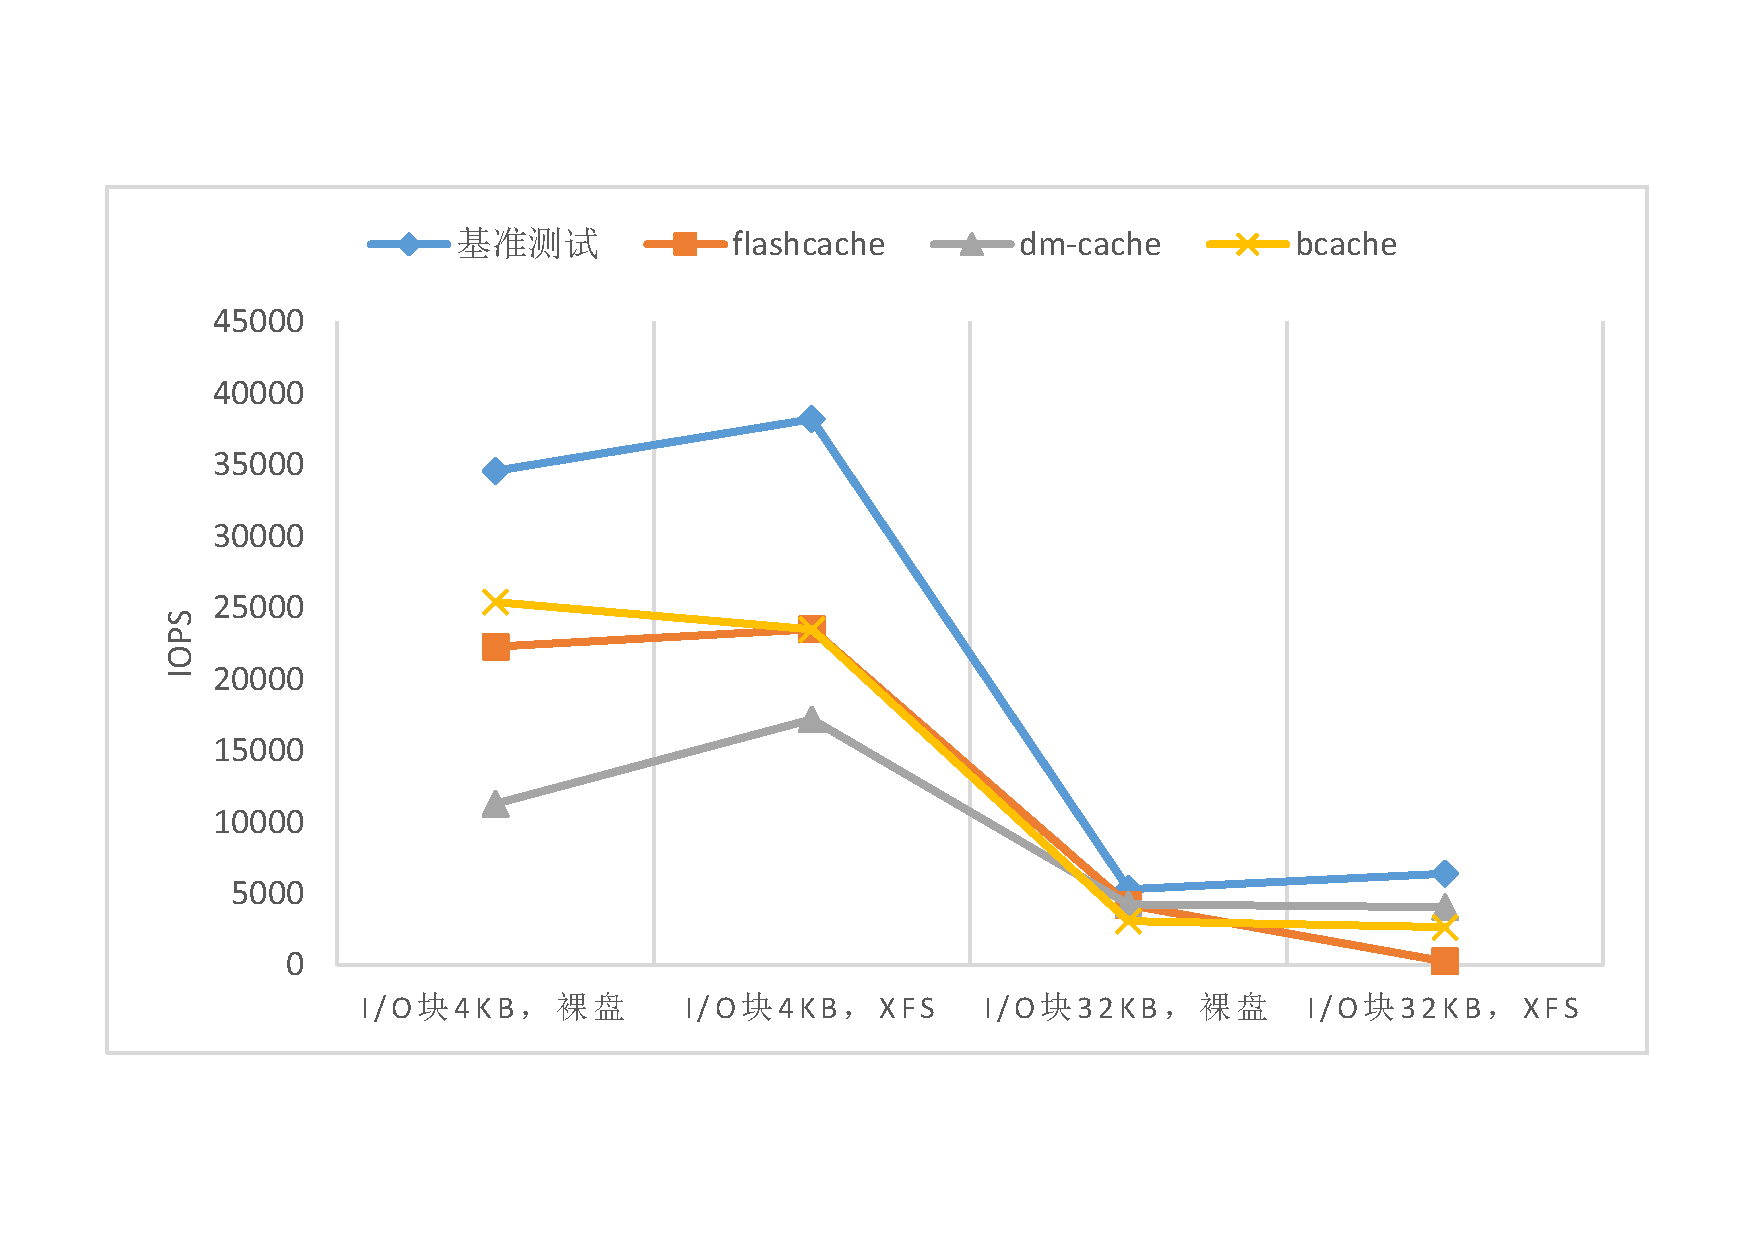
\includegraphics[width=0.7\textwidth]{opensource_randread.pdf}
    \bicaption[fig:opensource_randread]{基准测试、flashcache、dm-cache、bcache随机读性能对比}{基准测试、flashcache、dm-cache、bcache随机读性能对比}{Fig.}{comparison of random read among standard, flashcache, dm-cache and bcache}
\end{figure}

随机写性能对比图如图\ref{fig:opensource_randwrite}所示。可以看到相比随机读性能,flashcache、dm-cache和bcache三者的差距在小I/O时拉的更开,而在大I/O块时同样性能比较接近。与随机读不同,在随机写时,bcache的性能总体与SSD的性能持平,这是由于bcache采用日志追加的方式进行写操作处理,因此在小I/O块时性能非常优异。

\begin{figure}[H]
    \centering
    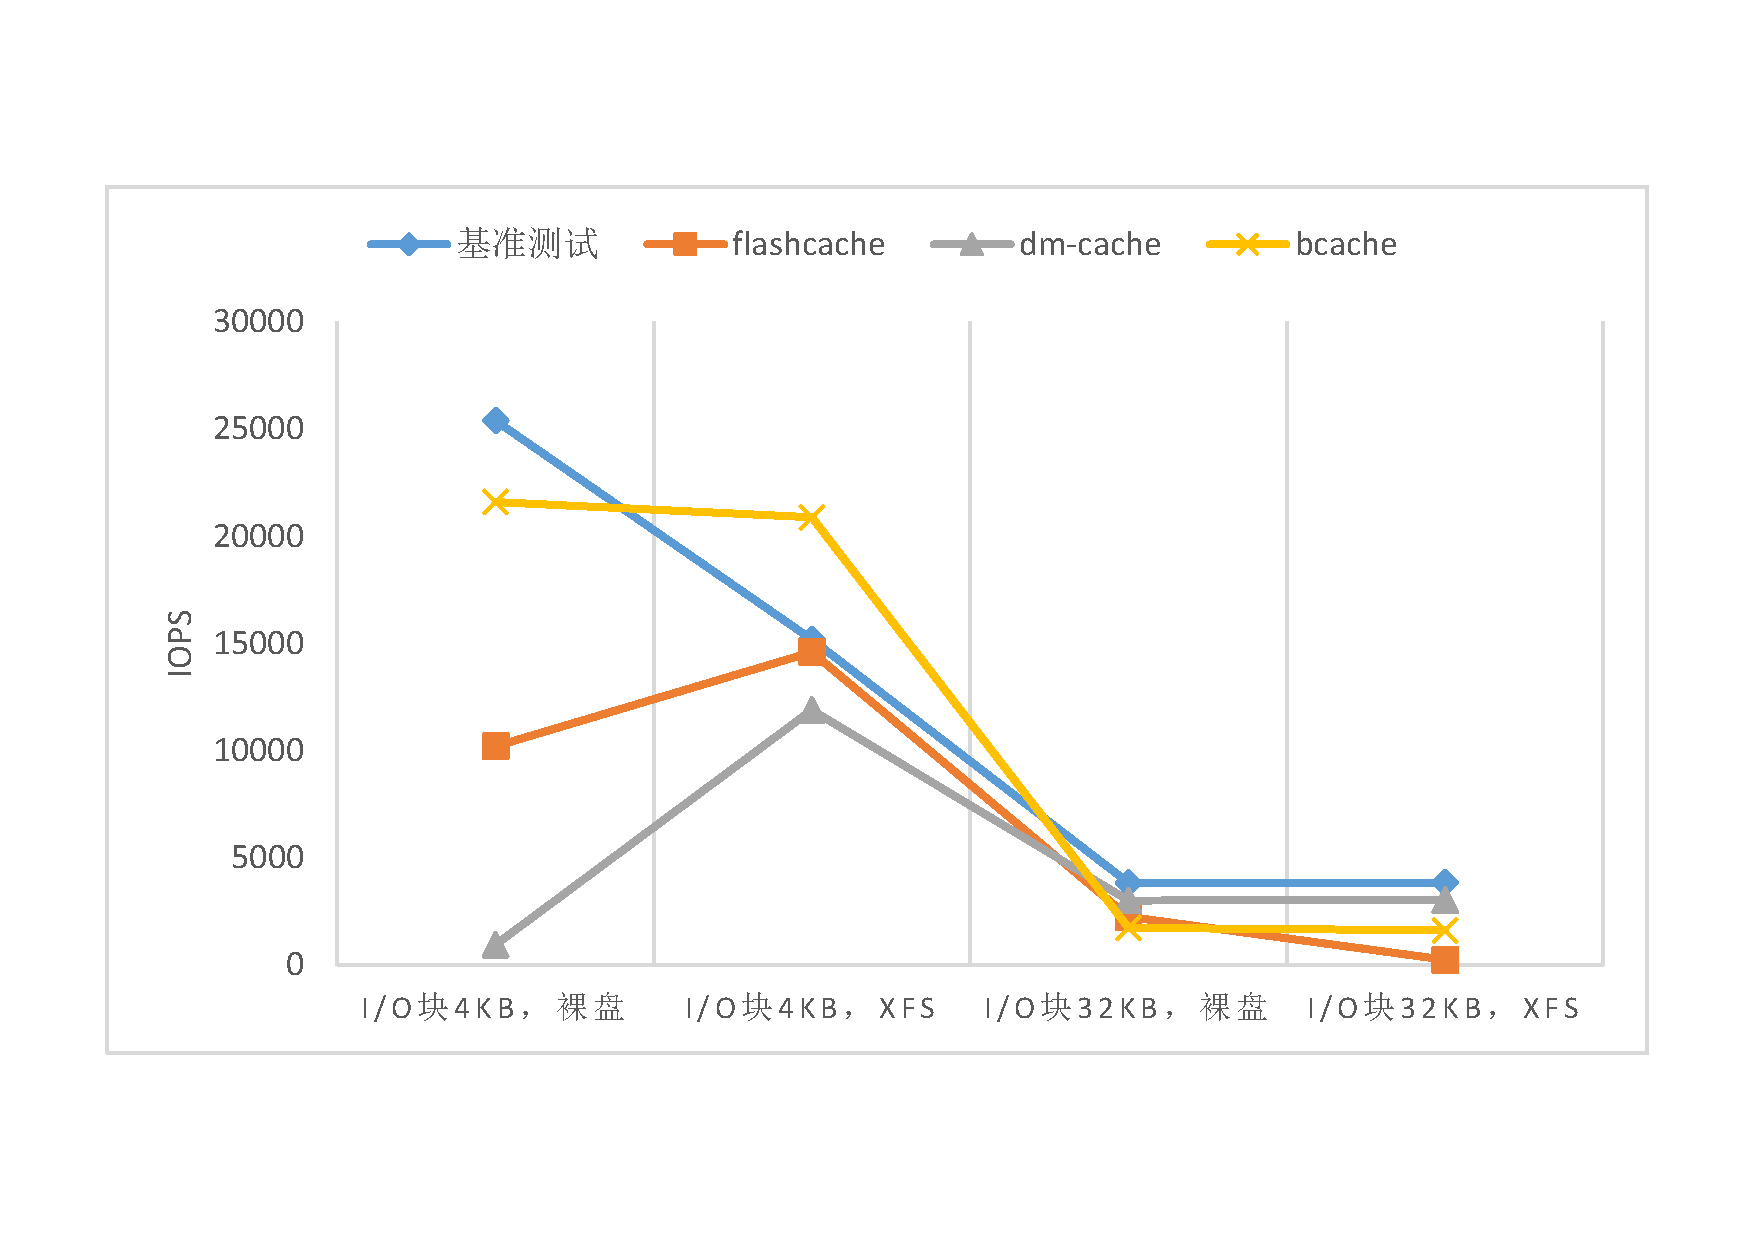
\includegraphics[width=0.7\textwidth]{opensource_randwrite.pdf}
    \bicaption[fig:opensource_randwrite]{基准测试、flashcache、dm-cache、bcache随机写性能对比}{基准测试、flashcache、dm-cache、bcache随机写性能对比}{Fig.}{comparison of random write among standard, flashcache, dm-cache and bcache}
\end{figure}

混合随机读写性能对比图如图\ref{fig:opensource_randrw_read}和图\ref{fig:opensource_randrw_write}所示。可以看到总体趋势仍然是在小I/O块时flashcache、dm-cache、bcache的性能差距会比较大,在大I/O块时性能则都很接近。并且总的来看,混合随机读写下,读性能与写性能几乎一样。与单纯的随机读或随机写性能差距较大的是bcache,在混合随机读写下bcache在小I/O块且使用XFS文件系统时性能有极具衰减。

\begin{figure}[H]
    \centering
    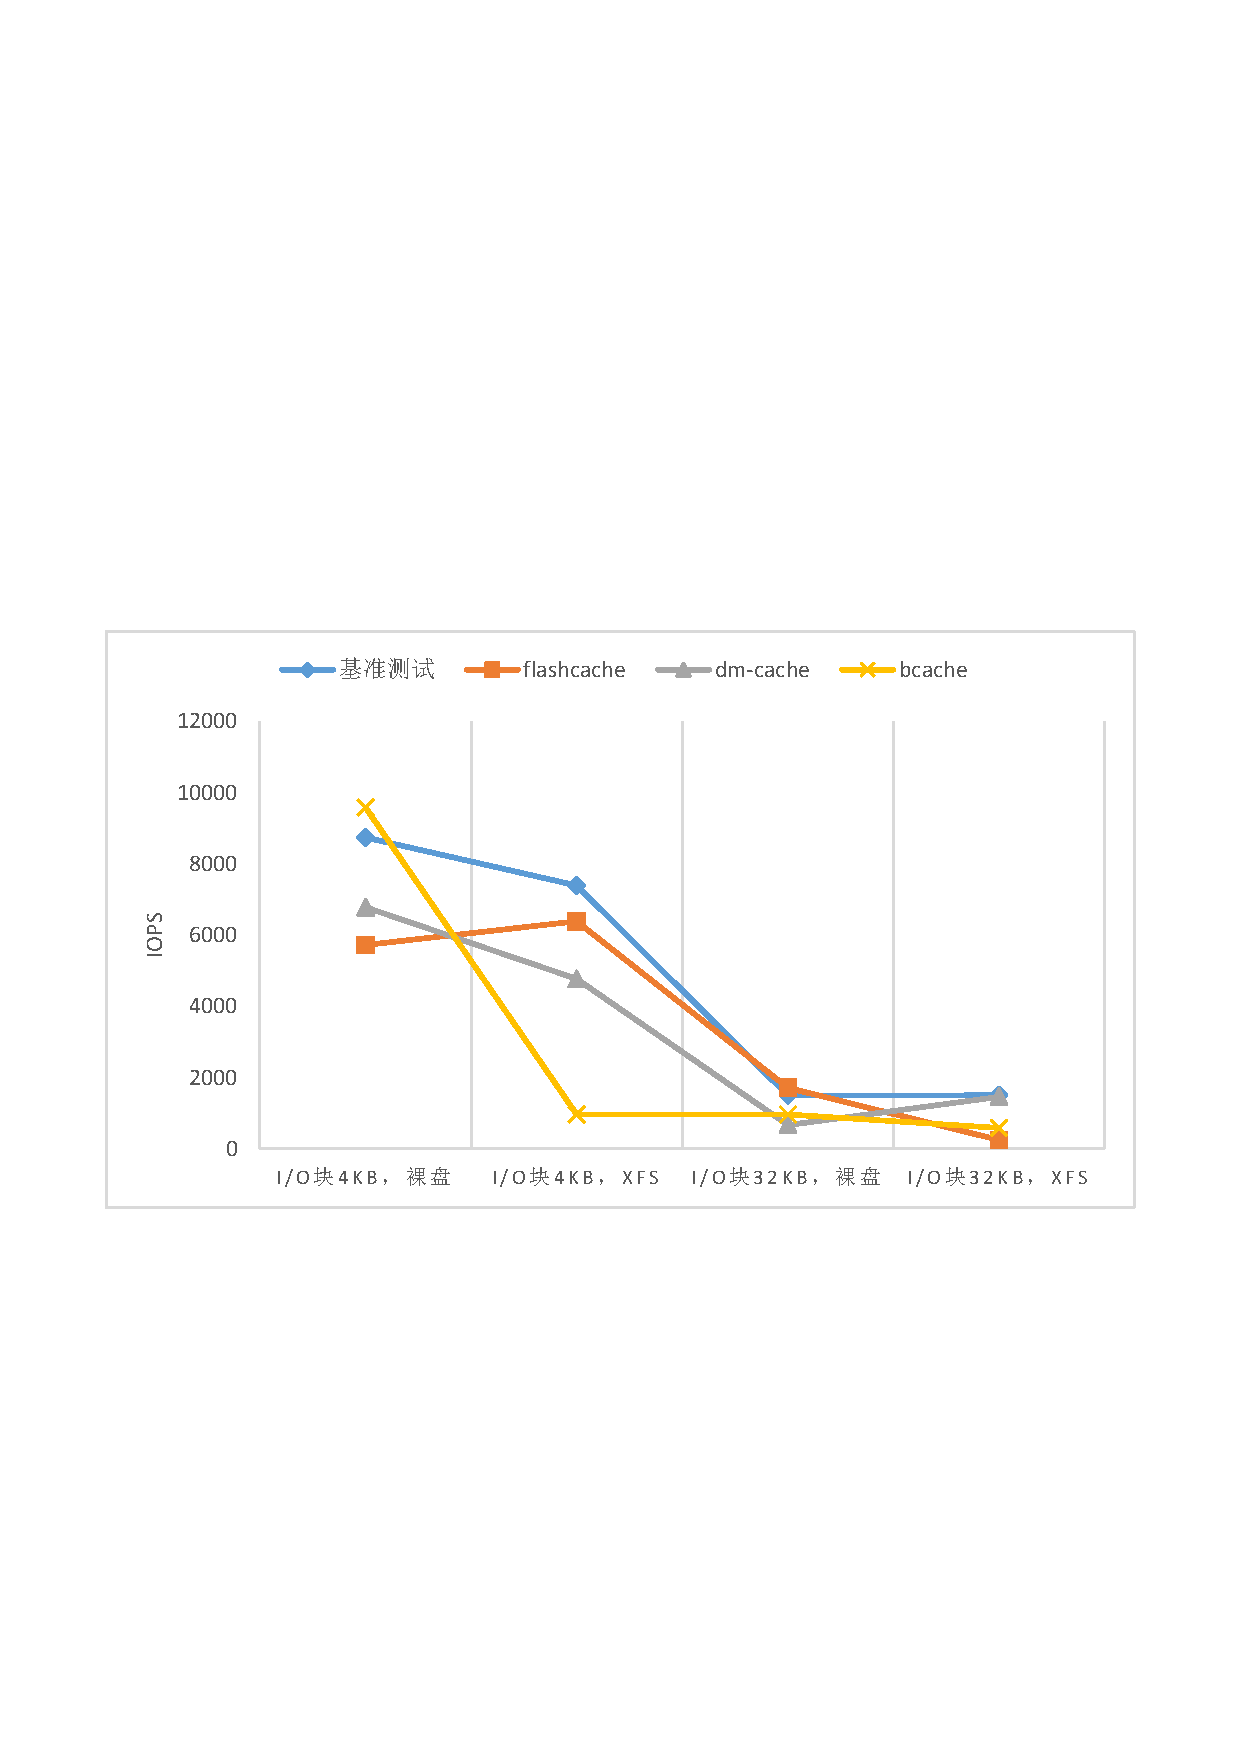
\includegraphics[width=0.7\textwidth]{opensource_randrw_read.pdf}
    \bicaption[fig:opensource_randrw_read]{基准测试、flashcache、dm-cache、bcache混合随机读写中读性能对比}{基准测试、flashcache、dm-cache、bcache混合随机读写中读性能对比}{Fig.}{comparison of random read/write read among standard, flashcache, dm-cache and bcache}
\end{figure}

\begin{figure}[H]
    \centering
    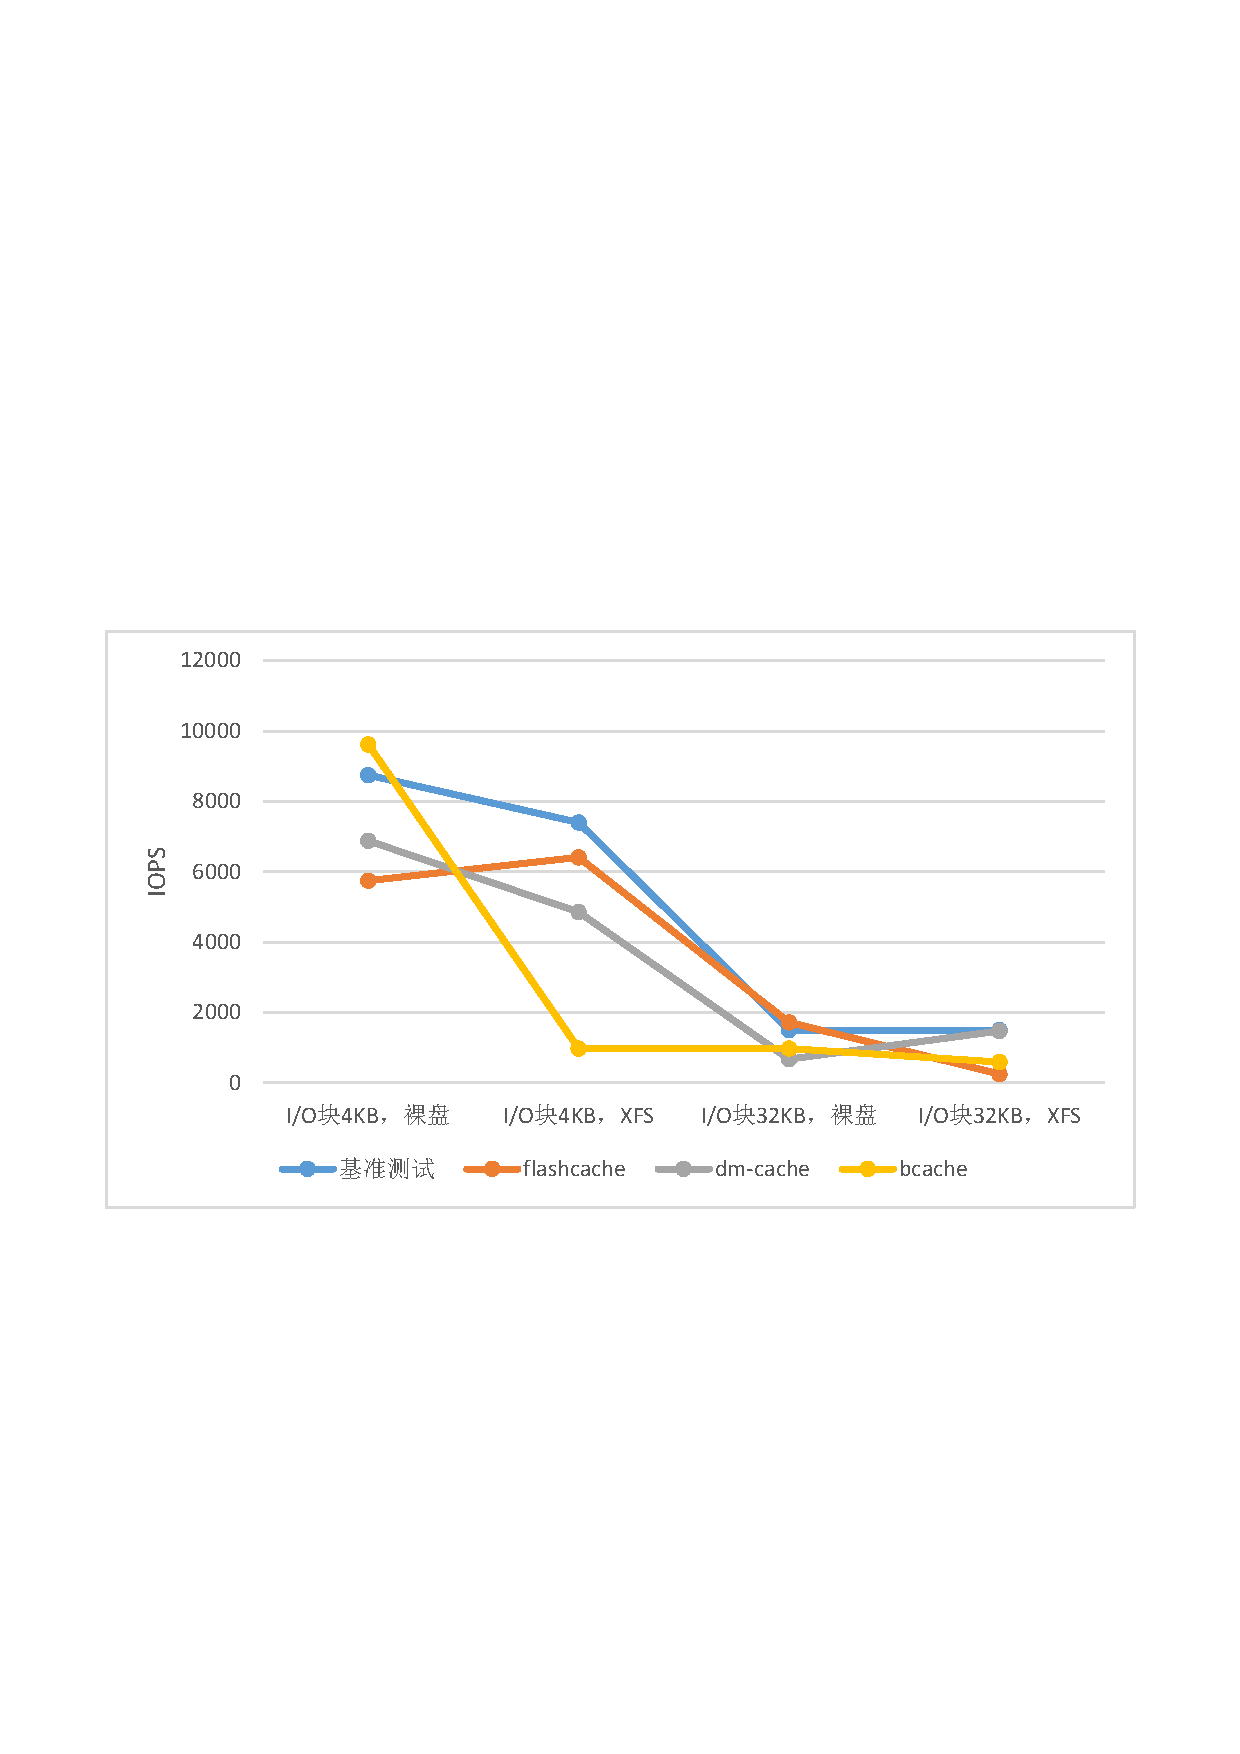
\includegraphics[width=0.7\textwidth]{opensource_randrw_write.pdf}
    \bicaption[fig:opensource_randrw_write]{基准测试、flashcache、dm-cache、bcache混合随机读写中写性能对比}{基准测试、flashcache、dm-cache、bcache混合随机读写中写性能对比}{Fig.}{comparison of random read/write write among standard, flashcache, dm-cache and bcache}
\end{figure}

\section{本章小结}

本章从上章提到的混合存储系统设计中系统架构、数据映射策略、冷热数据识别策略、数据写回/迁移策略、最优化存储设备组合这五个方面对现有三个开源混合存储系统flashcache、dm-cache、bcache进行了分析,并且经过测试给出了flashcache、dm-cache、bcache的特性对比以及性能对比。从特性对比来看flashcache在可靠性方面优于另两者,bcache在内存消耗方面有较大不足。从性能测试来看flashcache的缓存要求非常严格,必须设备边界对齐且长度一致才能被缓存,dm-cache和bcache则没这个限制。在I/O块4k时bcache表现优异,但是在大I/O块时表现不如flashcache和dm-cache。当缓存命中率接近100\%时,flashcache性能要略优于dm-cache。